\chapter{Wstęp}
\section{Cel projektu}

Celem projektu jest ukazanie oraz dokonanie pomiarów zmienności rzeczywistych sieci systemów autonomicznych. Sieci te są reprezentowane za pomocą grafów nieskierowanych. Do ich analizy zastosowano algorytmy typowo wykorzystywane w przypadku badania sieci społecznościowych, tak zwane miary centralności grafu. Oprócz nich szczególną uwagę zwrócono na stopień poszczególnych węzłów.

\section{Systemy autonomiczne}
Oryginalnie projekt miał opierać się na analizie grafów, gdzie każdy wierzchołek odpowiadał pojedynczemu urządzeniu - routerowi. Ze względu jednak na niską dostępność takich zestawów danych oraz ich gigantyczny rozmiar (niemożliwy do przetworzenia na dostępnym sprzęcie), zdecydowano się na badanie większych jednostek. System autonomiczny to sieć lub grupa sieci opartych na protokole IP pod wspólną administracyjną kontrolą, w której utrzymywany jest spójny schemat trasowania. Struktury te są podstawową jednostką budulcową Internetu na poziomie domen. Większość dostępnych topologii sieci internetowej opiera się na ich strukturze, dlatego uznano, że i w opisywanym projekcie znajdą zastosowanie.

\section{Dane sieci}

Znalezienie odpowiednich danych wejściowych wymagało trochę czasu. Z racji niedeterministycznej struktury badanych sieci, niemożliwe było wygenerowanie danych testowych. Konieczne okazało się wykorzystanie danych pochodzących z badań istniejącej sieci internetu. Zdecydowano się wykorzystać zestaw pochodzący z projektu University of Oregon Route Views. Zawiera on 733 instancje grafu, tworzonego poprzez codzienne badania struktury sieci na poziomie systemów autonomicznych. Najstarsza instancja pochodzi z 8 listopada 1997 roku, najmłodsza z 2 stycznia 2000 roku. Dane były zbierane za pomocą techniki multi-hop z wykorzystaniem protokołu BGP.  

\section{Wstępne przygotowanie danych}

Dane zawarte w zestawie mają postać listy krawędzi. Mimo iż są to grafy nieskierowane, wszystkie krawędzie występują w postaci zdublowanej oraz część węzłów posiada pętle. Warto tu nadmienić, że taki zapis grafu w pewnym kontekście na pewno miał określone znaczenie. Jednakże z punktu widzenia zamierzonych badań oba zjawiska były niepożądane, w związku z czym napisano własną funkcję wczytującą graf do programu. Jej zadaniem było odfiltrowanie krawędzi wielokrotnych oraz pętli. 

Drugim problemem na który natknięto się po wczytaniu grafów, były duże błędy pomiarowe. Po stworzeniu wykresu liczby wierzchołków dla wszystkich instancji zauważono, że istotna ich część znacząco odstaje od widocznego trendu (w kierunku zera). Wykres liczby krawędzi ukazał spadki w tych samych miejscach, co utwierdziło autorów o błędach w pomiarach. Podejrzewają oni, że było to spowodowane przerwaniem procesu zbierania danych o strukturze sieci. Zaskutkowało to mniejszymi instancjami grafów dla niektórych  dni. W celu ujednolicenia danych zastosowano funkcję usuwającą obserwacje odstające zawartą w oprogramowaniu Matlab \textit{isoutlier()}. Efekt jej działania można zobaczyć poniżej.

\begin{figure}[h]
	\centering
	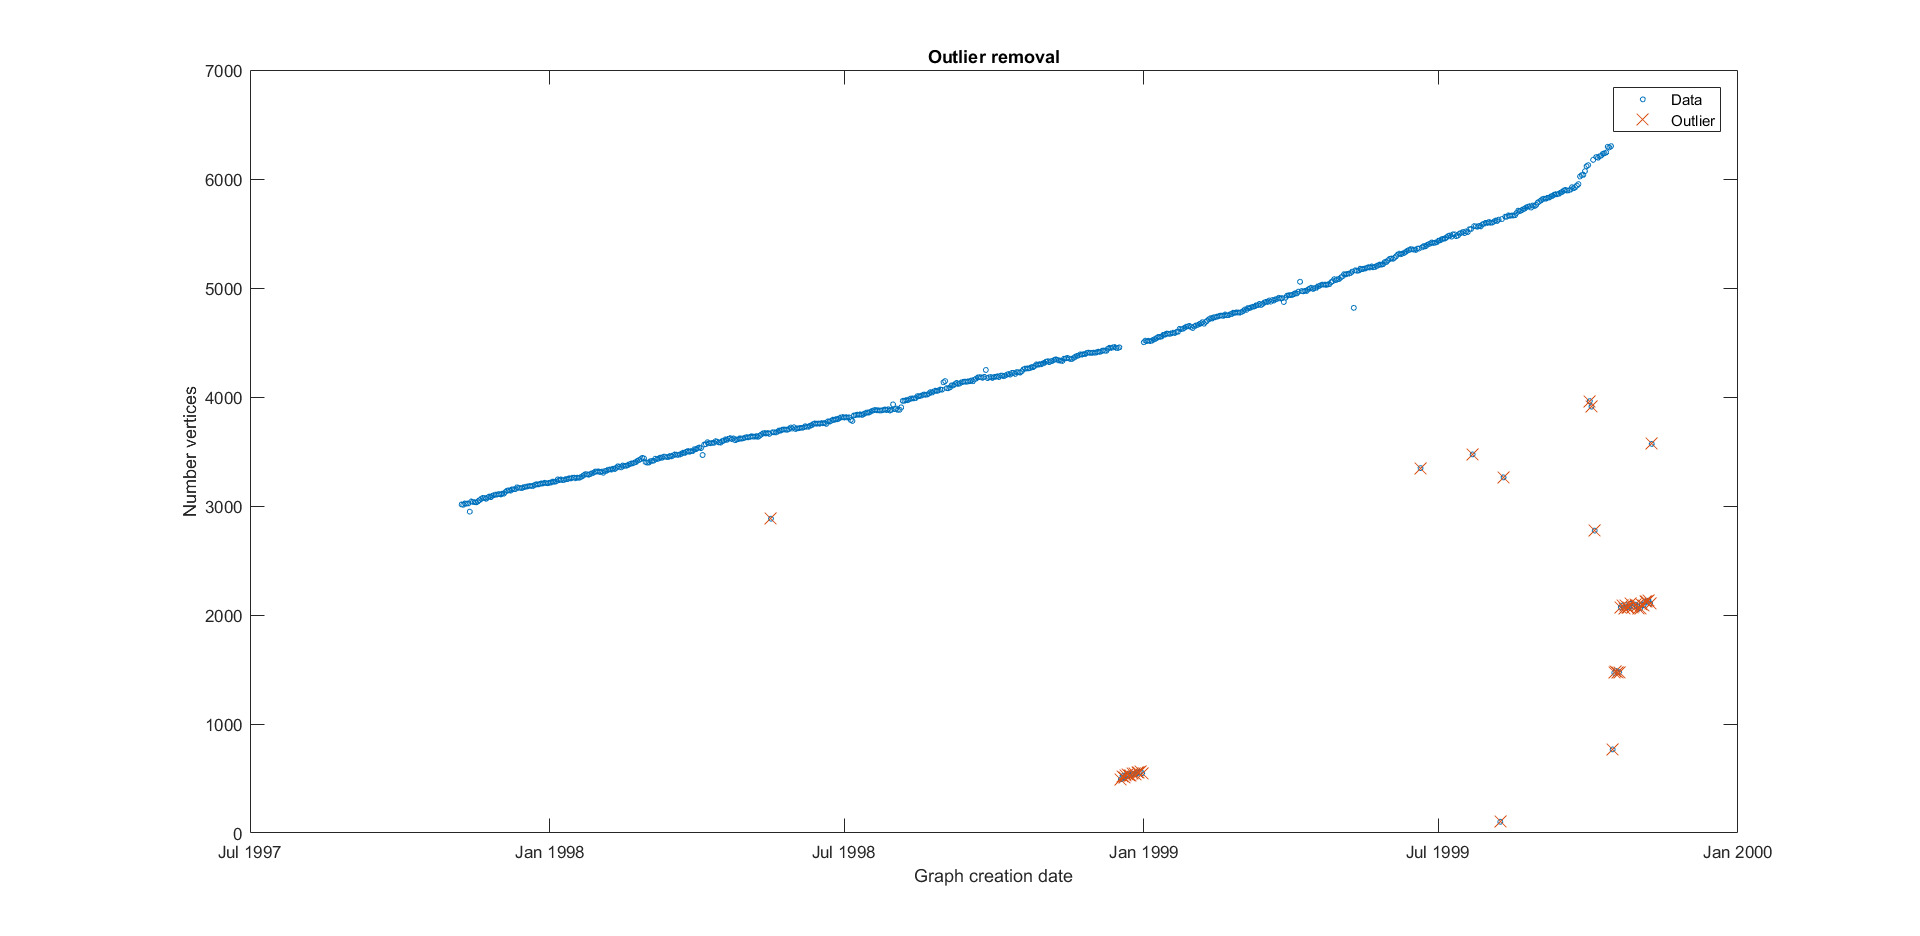
\includegraphics[width=\textwidth]{Outliers}
	\caption{Wykres liczby wierzchołków dla poszczególnych instancji z zaznaczonymi obserwacjami odstającymi}
\end{figure}


